\chapter{Marco Teórico}
\label{chap:marcoteorico}

% Estado del arte general de la temática de estudio. 
\begin{itemize}
 \item CDM: Recepci\'on.
 \item Metodolog\'ia Akella \& Alfriend.
 \item Metodolog\'ia Osweiler.
\end{itemize}

\subsection{CDM}
(JAC SW - Laporte)

{\bf{CSM:}} They are made available on Emergency Criteria, wich are Time of Closest Approach whithin 72 hs combined with a miss distance criteria:\\
LEO:\\
overall miss distance < 1km\\
radial miss distance < 200m\\
GEO/MEO:\\
Overall miss distance < 10 km.\\

CSM are advisory and informational messages only and are not directly actionable. They don´t provide a direct recommendation to perform an avoidance action and of course they cannot take neither the operational constraints of the asset nor the maneuvers the asset plansor just performed. (sigue ver apuntes Laporte carpeta...)\\

!!! JSpOC NO CUENTA CON INFORMACI\'ON DE MANIOBRAS PLANIFICADAS, puede haber falsas alarmas.\\

CONCEPTO DE MIDDLE MAN.\\
CONCEPTO DE COLLABORATIVE WORK ENVIRONMENT. (close loop process)

Con el creciente avance de la tecnolog\'ia y el acceso al espacio, aumenta la poblaci\'on de objetos que orbitan la Tierra, ya sean  misiones operativas o desechos espaciales. Con esta perspectiva, varios estudios alertan que las colisiones en \'orbita podr\'ian convertirse en las principales fuentes de generaci\'on de nuevos desechos espaciales. \cite{KlinkradChapter8}\\

Dado el car\'acter global de esta problem\'atica, distintas naciones y agencias internacionales con gran desarrollo y actividad espacial, se han estado organizado en la b\'usqueda de acuerdos y buenas pr\'acticas. Entre los organismos que coordinan las recomendaciones, se encuentran:\\

\begin{itemize}
\item {\small{COPUOS: Committee of the Peacefull Uses of Outer Space (ONU)}}
\item {\small{IADC: Inter-Agency Space Debris Coordination Committee}}
\item {\small{CCSDS: Consultative Committee for Space Data Systems}}
\end{itemize}

As\'i mismo, en lo que respecta a los l\'imites de este trabajo, podemos citar las siguientes Normas, Recomendaciones y Legislaci\'on:\\

\begin{itemize}
\item {\small{Convenio sobre Responsabilidad Internacional por da\~nos causados por objetos espaciales. ONU - (29-03-72)}}
\item {\small{Ley 23.335 (19-08-86) - Arg. Suscribe al Convenio de ONU.}}
\item {\small{Space Debris Mitigation Guidelines - IADC}}
\item {\small{ISO 24113:2011 {\it{Space Debris mitigation requirements}}}}
\item {\small{ISO/TR 16158:2013 {\it{Space Systems - Avoiding collision with orbiting objects}}}}
\item {\small{ISO 19389:2014 {\it{Space data and information transfer Systems}}}}

\end{itemize}


En este contexto, ya existen claros antecedentes que abordan la problem\'atica con sus respectivos soportes inform\'aticos. (ver tabla \ref{tab:sisal})
\begin{table}[!h]
\centering
\begin{tabular}{|l|p{5cm}|p{6cm}|}
\hline
Herramienta & Desecripci\'on & Proveedor/Agencia\\
\hline
{\bf{CARA}} & {\it{Conjunction Assessment Risk Analysis}} & NASA Robotic Conjunction Assessment Risk Analysis group, en convenio con la empresa a.i. solutions, Inc.\\
\hline
{\bf{SOCRATES}} & {\it{Satellite Orbital Conjuction Reports Assessing Threatening Encounters in Space}}, servicio web v\'ia Celestrack.com & CSSI (Center for Space Standards \& Innovation) de la agencia AGI: Analytical Graphics, Inc.\\
\hline
{\bf{CRASS}} & {\it{Collision Risk Assessment tool}} & Desarrollado por la
empresa GMV, que presta servicios al Centro Europeo de Operaciones
Espaciales (ESOC) - Darmstadt, Alemania. \cite{alarconRodriguez}\\
\hline
{\bf{CAESAR}} & {\it{Conjuction Analysis and Evaluation Service, Alerts and Recommendations}} & Agencia francesa CNES, que utiliza como soporte el Software JAC {\it{Java for Assessment of Conjunctions}}.\cite{laporte}\\
%\hline
%closeap - ant\'on & & ESA\\
\hline
{\bf{CRAMS}} & {\it{Collision Risk Assessment and Mitigation System}} & Canadian Space Agency (CSA). \cite{babiker}\\
\hline
\end{tabular}
\caption[Sistemas de Alerta]{Sistemas de Alertas de distintas Naciones y Agencias}
\label{tab:sisal}
\end{table}

\subsection*{El Estudio de Riesgo de Colisi\'on}
El estudio de riesgo de colisi\'on se basa en la capacidad de determinar y predecir las \'orbitas de los objetos involucrados en un acercamiento con la mayor precisi\'on posible.\\
Las {\bf{misiones operativas}} permiten conocer la posici\'on de la nave ya sea por sistemas de navegaci\'on como GPS, Doppler, etc. y por determinaciones orbitales a posteriori, de las que se desprenden los errores asociados a la posici\'on.\\
En el caso de los {\bf{desechos espaciales}} la situaci\'on es muy diferente. La \'unica informaci\'on de la posici\'on con la que se cuenta, la suministran las agencias de rastreo, ya que el desecho no tiene capacidades funcionales que le permitan enviar informaci\'on.\\

Existe hoy un \'unico organismo que rastrea permanentemente y publica diariamente las posiciones de todos los objetos catalogados, es el \ac{NORAD}. De modo que todas las agencias o paises que no cuentan con capacidad suficiente de rastreo, como es el caso de CONAE, se encuentran sujetas a la informaci\'on que provee NORAD y a los servicios de alerta contratados u acordados por distintos convenios.\\
Si bien \ac{NORAD} ofrece v\'ia su p\'agina SPACE-TRACK{\footnote{http://www.space-track.org}} los datos de todos los objetos rastreados que orbitan la Tierra (en formato de \ac{TLE}) y el modelo de propagaci\'on \ac{SGP4}, los mismos no informan los errores asociados a la medici\'on y la estimaci\'on de la posici\'on publicada. \\
De modo que si uno quisiera hacer uso de esa informaci\'on para predecir situaciones de encuentro, o analizar situaciones ya alertadas, se ve obligado a buscar herramientas de estimaci\'on de los errores que se cometen al utilizar los TLE para propagar y predecir la posici\'on del desecho espacial hasta el momento de la situaci\'on del encuentro.\\ 

Dado este contexto, las distintas agencias, que no cuentan con gran n\'umero de misiones operativas, suelen contratar/acordar este servicio. Y a\'un, con herramientas propias desarrolladas, lleva tiempo la validaci\'on de las mismas hasta lograr cierta autonom\'ia. No obstante, la tendencia es hacia un primer paso, que permita una caracterizaci\'on m\'as precisa de la situaci\'on de encuentro, sumando a la informaci\'on p\'ublica, m\'etodos de ajuste, datos propios de la misi\'on en riesgo y estimadores del riesgo como por ejemplo la \ac{PoC}.\\
Es en esa direcci\'on que planteamos este trabajo, a fin de ofrecer un prototipo que pueda ser implementado en paralelo a lo que ya se utiliza en CONAE, para ser probado y mejorado con la experiencia que sumen los encuentros que involucren a las misiones nacionales.\\

\subsection*{ARxCODE}
El ARxCODE es una aplicaci\'on de b\'usqueda y detecci\'on de archivos CDM para el procesamiento y an\'alisis de situaciones de riesgo por colisi\'on, que contar\'a con las siguientes capacidades:

\begin{itemize}
\item Extraer la informaci\'on que provee el CDM.
\item Propagar la posici\'on del desecho espacial involucrado con un m\'etodo de estimaci\'on del error.
\item Solicitar al operador/analista experto de Din\'amica Orbital las posiciones precisas de la misi\'on en riesgo.
\item Calcular la probabilidad de colisi\'on del encuentro.
\item Permitir al operador/analista experto visualizar el encuentro, generar reportes y notificaciones.
\end{itemize} 


\begin{figure}[!h]
  \centering
  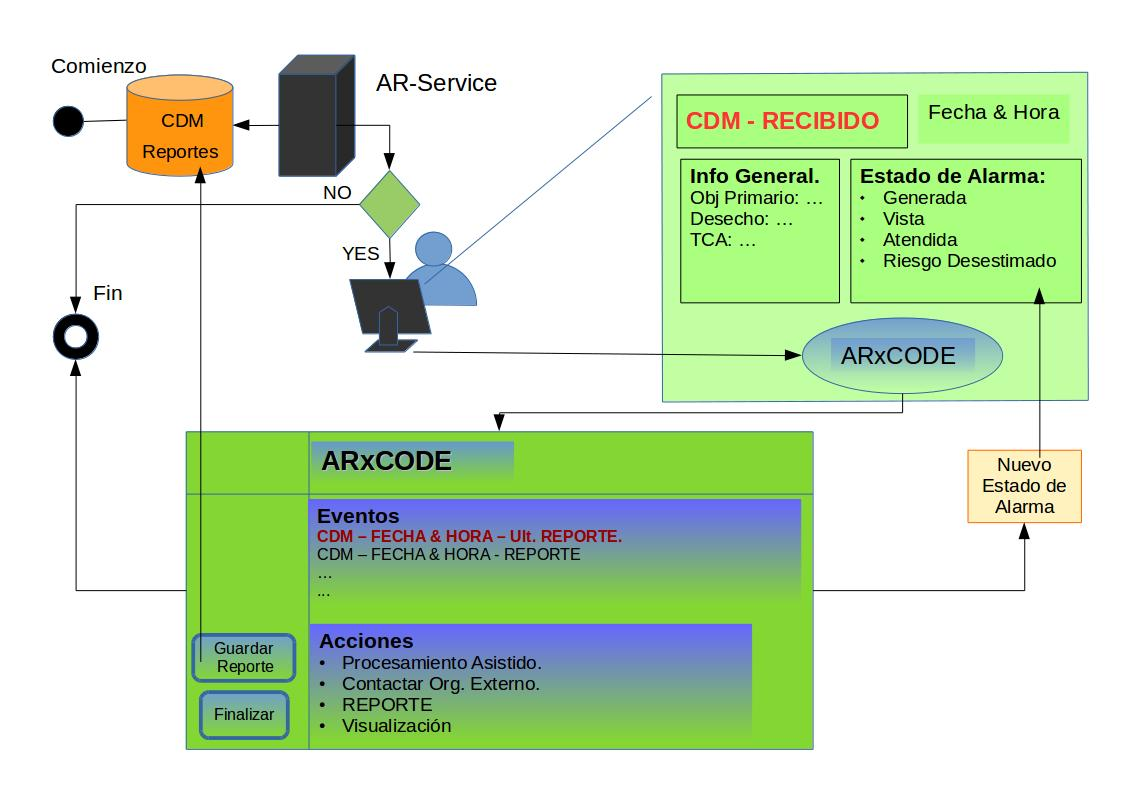
\includegraphics[width=0.8\textwidth]{imagenes/ARprocedimiento}
\end{figure}

\subsection*{Arquitectura y Dise\~no Preliminar}
El prototipo de software para el An\'alisis de Riesgo por Colisi\'on con Desechos Espaciales {\it{ARxCODE}}, ser\'a un sistema anexo a las estructuras ya existentes dentro del departamento de Din\'amica Orbital.\\
Ocupa un rol de intermediario a fin de facilitarle a un operador analista experto, herramientas para la toma de decisiones o el intercambio de informaci\'on con los organismos externos y el centro de control.\\



\subsection*{Requerimientos}
\begin{itemize}
\item La aplicaci\'on detectar\'a la llegada de un CDM y ser\'a capaz de desglosarlo para extraer la informaci\'on que sea necesaria.\\
\item La aplicaci\'on identificar\'a los objetos y solicitar\'a al operador/analista experto la posici\'on precisa y la matriz varianza-covarianza en el caso de la misi\'on principal\\
\item La aplicaci\'on extraer\'a los TLEs del intervalo necesario a la p\'agina Space-Track, en el caso del desecho espacial.\\
\item La aplicaci\'on ajustar\'a la precisi\'on de la posici\'on del desecho espacial y generar\'a la matriz de varianza-covarianza para el mismo.\\
\item La aplicaci\'on calcular\'a la PoC.\\
\item La aplicaci\'on tendr\'a la capacidad de generar reportes, notificaciones y visualizaciones para facilitar la comprensi\'on y el an\'alisis del riesgo.
\item La aplicaci\'on deber\'a funcionar 7x24.
\end{itemize}

\subsubsection*{Funcionalidades:}
\begin{itemize}
\item Detectar la recepi\'on de un nuevo mensaje de alerta.\\
\item Extraer la informaci\'on del mensaje y adaptarla al formato necesario.\\
\item Extraer de la web (via spacetrack) los TLE del desecho espacial involucrado.\\
\item Solicitar al operador/analista experto la posici\'on precisa de la misi\'on primaria y el error asociado.\\
\item Propagar y ajustar la posici\'on del desecho al instante del acercamiento, con su error asosciado\\
\item Calcular la PoC.\\
\item Generar reportes, notificaciones y visualizaciones.\\
\end{itemize}


